\documentclass{scrartcl}
\usepackage{wallpaper}
\usepackage{amsmath}
\usepackage{mathpazo}
\usepackage{helvet}
\renewcommand{\ttdefault}{cmtt}
\usepackage{newtxmath}
\usepackage[T2A,T1]{fontenc}
\usepackage[utf8]{inputenc}
\usepackage{tipa}
\usepackage{tipx}
%% ----------------------------------------------------------------------------
%% Book Parameters - Included in body and cover
%% ----------------------------------------------------------------------------
\usepackage{pgf}% Fancy math

% Note that some printers require specific page count multiples:
% -- Createspace: page count MUST be divisible by 2.
% -- Ingram: page count MUST be divisible by 2.
% -- Blurb : page count MUST be divisible by 6.
% Add blank pages as needed in final PDF generations!
\pgfmathsetmacro\TotalPageCount{672}% Must be manually entered
\pgfmathsetmacro\PaperWidthPt{7.444in}%
\pgfmathsetmacro\PaperHeightPt{9.68in}%

%% ----------------------------------------------------------------------------
%% Computed parameters for cover and jacket design 

% CreateSpace and Ingram, use different paper stock so the spine width must
% be adjusted to refect that. 
% For example Createspace, White paper: multiply page count by 0.002252
%
% Use Createspace parameters for Lulu.com
\pgfmathsetmacro\SinglePageThicknessPt{0.002252in}% Createspace, White B&W Paper
%\pgfmathsetmacro\SinglePageThicknessPt{0.002143in}% Blurb, Standard and Economy B&W Paper
%\pgfmathsetmacro\SinglePageThicknessPt{0.002602in}% Blurb, Standard and Economy Color Paper
%\pgfmathsetmacro\SinglePageThicknessPt{0.002110in}% Ingram, Standard White B&W Paper (50lb)
%\pgfmathsetmacro\SinglePageThicknessPt{0.002110in}% Ingram, Standard Color Paper (50lb)
%\pgfmathsetmacro\SinglePageThicknessPt{0.002720in}% Ingram, Premium Color Paper (70lb)

\pgfmathsetmacro\HorBleedPt{0.125in}%
\pgfmathsetmacro\VerBleedPt{0.125in}%
\pgfmathsetmacro\FoldVariancePt{0.0625in}%

%% Every book will vary slightly when bound. Allow for 0.0625" variance on either
%% side of the fold lines for your cover. For example, if your spine width is 1",
%% your text should be no wider than 0.875". Because of this variance, avoid hard
%% edges or lines that end on the fold line.

%% Cover Width calculation at 6" x 9" cover with 60 B&W pages on white paper:
%%    0.125" + 6" + (60 * 0.002252)" + 6" + .125" = 12.385"
%% Cover Height calculation: 6" x 9": 0.125" + 9" + .125" = 9.25"

\pgfmathsetmacro\SpineWidthPt{\SinglePageThicknessPt*\TotalPageCount}%
\pgfmathsetmacro\CoverWidthPt{\PaperWidthPt+\HorBleedPt}%
\pgfmathsetmacro\JacketWidthPt{\CoverWidthPt+\SpineWidthPt+\CoverWidthPt}%
\pgfmathsetmacro\CoverHeightPt{\VerBleedPt+\PaperHeightPt+\VerBleedPt}%

\pgfmathsetmacro\PtsPerInch{72.27}% Slightly more than 72 - odd.

\pgfmathsetmacro\SpineWidth{\SpineWidthPt    / \PtsPerInch}%
\pgfmathsetmacro\PaperWidth{\PaperWidthPt    / \PtsPerInch}%
\pgfmathsetmacro\CoverWidth{\CoverWidthPt    / \PtsPerInch}%
\pgfmathsetmacro\JacketWidth{\JacketWidthPt  / \PtsPerInch}%

\pgfmathsetmacro\PaperHeight{\PaperHeightPt  / \PtsPerInch}%
\pgfmathsetmacro\CoverHeight{\CoverHeightPt  / \PtsPerInch}%

\pgfmathsetmacro\HorBleed{\HorBleedPt        / \PtsPerInch}%
\pgfmathsetmacro\VerBleed{\VerBleedPt        / \PtsPerInch}%
\pgfmathsetmacro\FoldVariance{\FoldVariancePt/ \PtsPerInch}%
 
%% ----------------------------------------------------------------------------
%% End of Book Parameters.
%% ----------------------------------------------------------------------------

\usepackage{wrapfig}
\usepackage{geometry}
\usepackage{graphicx}
\usepackage{pagecolor}
\usepackage{changepage}

\geometry{
  paperwidth=\CoverWidth in,%
  paperheight=\CoverHeight in,%
  left=  0.5 in,%
  right= 1.0 in,%
  top=   0.8 in,%
  bottom=0.3 in,%
  footskip=0.0in%  
}

\pagestyle{empty}

%% ---------------------------------------------------------------------------
%% ---------------------------------------------------------------------------
\begin{document}
%\CenterWallPaper{1.01}{back-cover-background.jpg}
\begin{wrapfigure}{l}{0.312\columnwidth}
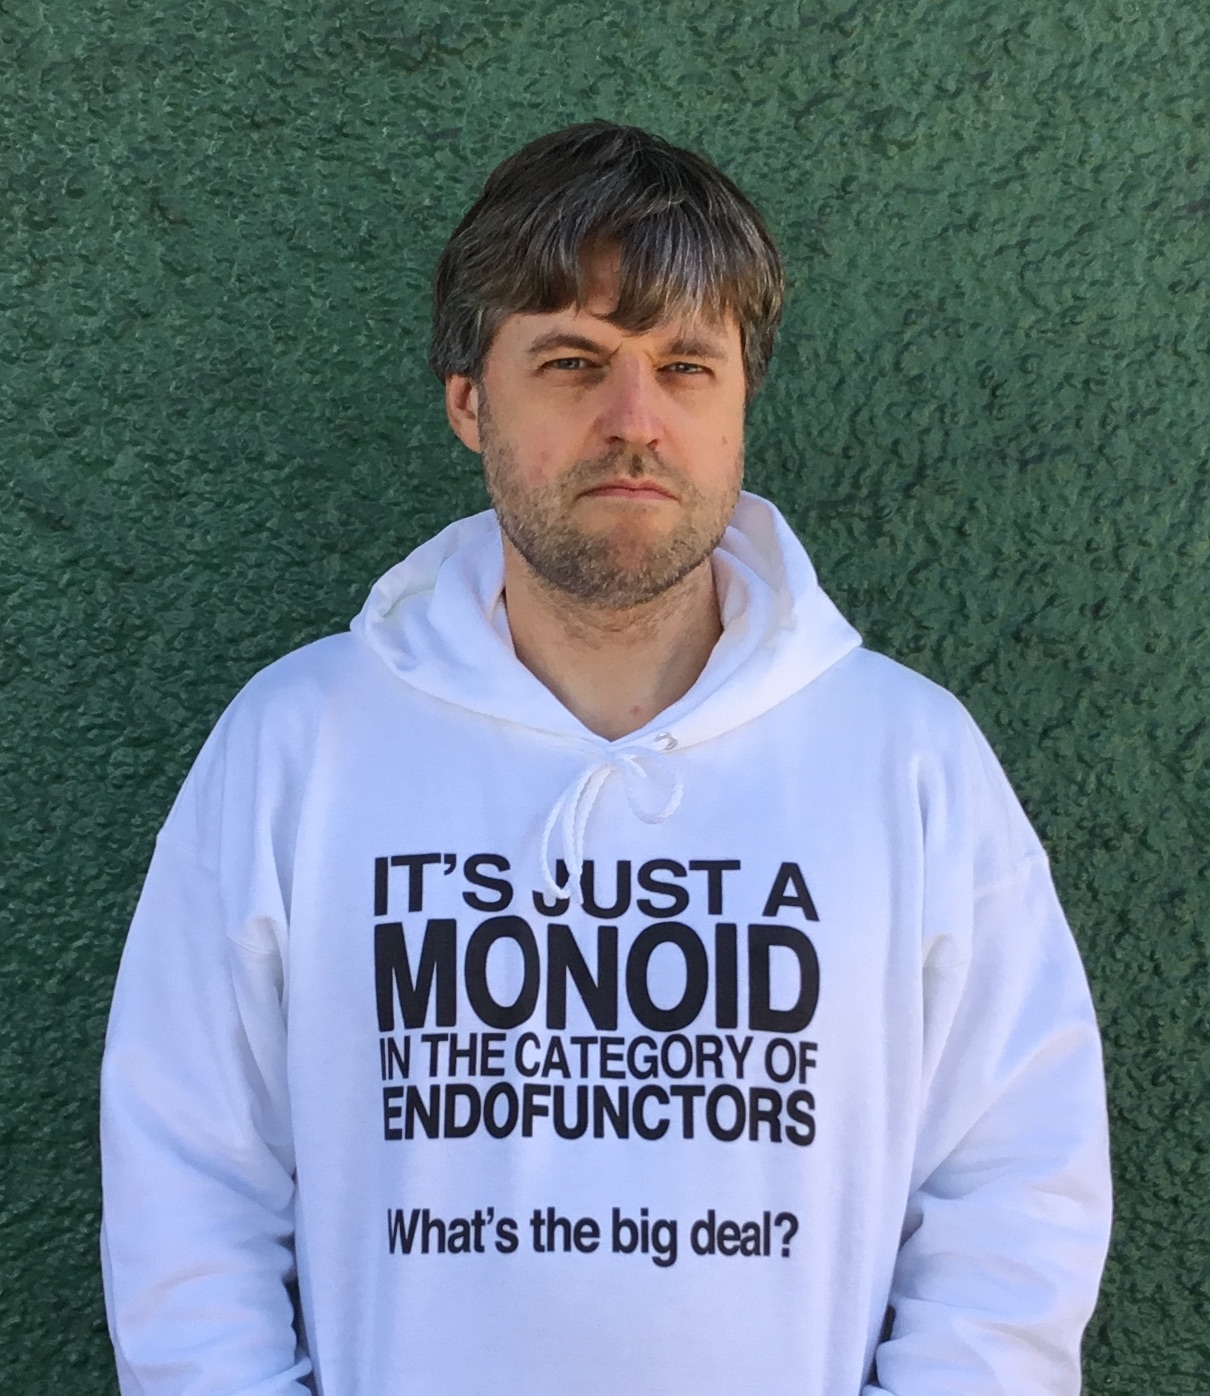
\includegraphics[width=0.312\columnwidth]{zloe-lico-monad.jpg}
\vspace{-2.4\baselineskip}
\end{wrapfigure}

\noindent
\large
This book is a pedagogical in-depth tutorial and reference
on the theory of functional programming (FP) as practiced in the early
21$^{\text{st}}$ century. Starting from issues found in practical
coding, the book builds up the theoretical intuition, knowledge, and
techniques that programmers need for rigorous reasoning about types
and code. Examples are given in Scala, but most of the material applies equally
to other FP languages.

The book's topics include working with collections; recursive
functions and types; the Curry-Howard correspondence; laws, structural
analysis, and code for functors, monads, and other typeclasses; techniques
of symbolic derivation and proof; parametricity theorems; and free
type constructions.

Long and difficult, yet boring explanations are logically
developed in excruciating detail and accompanied by 1481
Scala code snippets, 145 statements with step-by-step
derivations, 96 diagrams, 196 solved examples
with tested Scala code, and 223 exercises. Discussions
further build upon each chapter's material.

Beginners in FP will find clear explanations about the \texttt{map} / \texttt{reduce}
programming style, type parameters, disjunctive types, and higher-order
functions. For more advanced readers, the book shows  the practical
uses of the Curry-Howard correspondence and the parametricity theorems
without unnecessary jargon; proves that all the standard monads (e.g.,
\texttt{List} or \texttt{State})
satisfy the monad laws; derives lawful instances of \texttt{Functor}
and other typeclasses from types; shows that monad transformers need
18 laws; and explains the use of Yoneda identities for reasoning about
the Church encoding and the free type constructions.

Readers should have a working knowledge of programming; e.g.,
be able to write code that prints the number of distinct words in
a small text file. The difficulty of this book's mathematical derivations
is at the level of high-school calculus, similar to that of multiplying
matrices and simplifying the expressions
\[
\frac{1}{x-2}-\frac{1}{x+2}\quad\text{ and }\quad\frac{d}{dx}\left((x+1)f(x)e^{-x}\right)\quad.
\]

Sergei Winitzki received a Ph.D. in theoretical physics. After a career in academic research, he currently works as a software engineer.
\end{document}

